\chapter{Eksperimental Opsætning}
Denne sektion har til formål at beskrive opgavens eksperimentale opsætning og dertil, hvilke billeder, der er anvendt og hvordan metoderne er afprøvet.
\section{Anvendte Billeder}
Det udvalgte billedsæt, som opgavens resultater bygger på, er taget fra overflyvningen af én mark. Sættene består af: 11 billeder som er taget længst væk fra jorden, 6 billeder taget næst-længst fra jorden og 6 billeder taget tættest fra jorden. <I alle sættene er der traktorspor eller nedlagt korn.>
\begin{figure}[H]
    \centering
    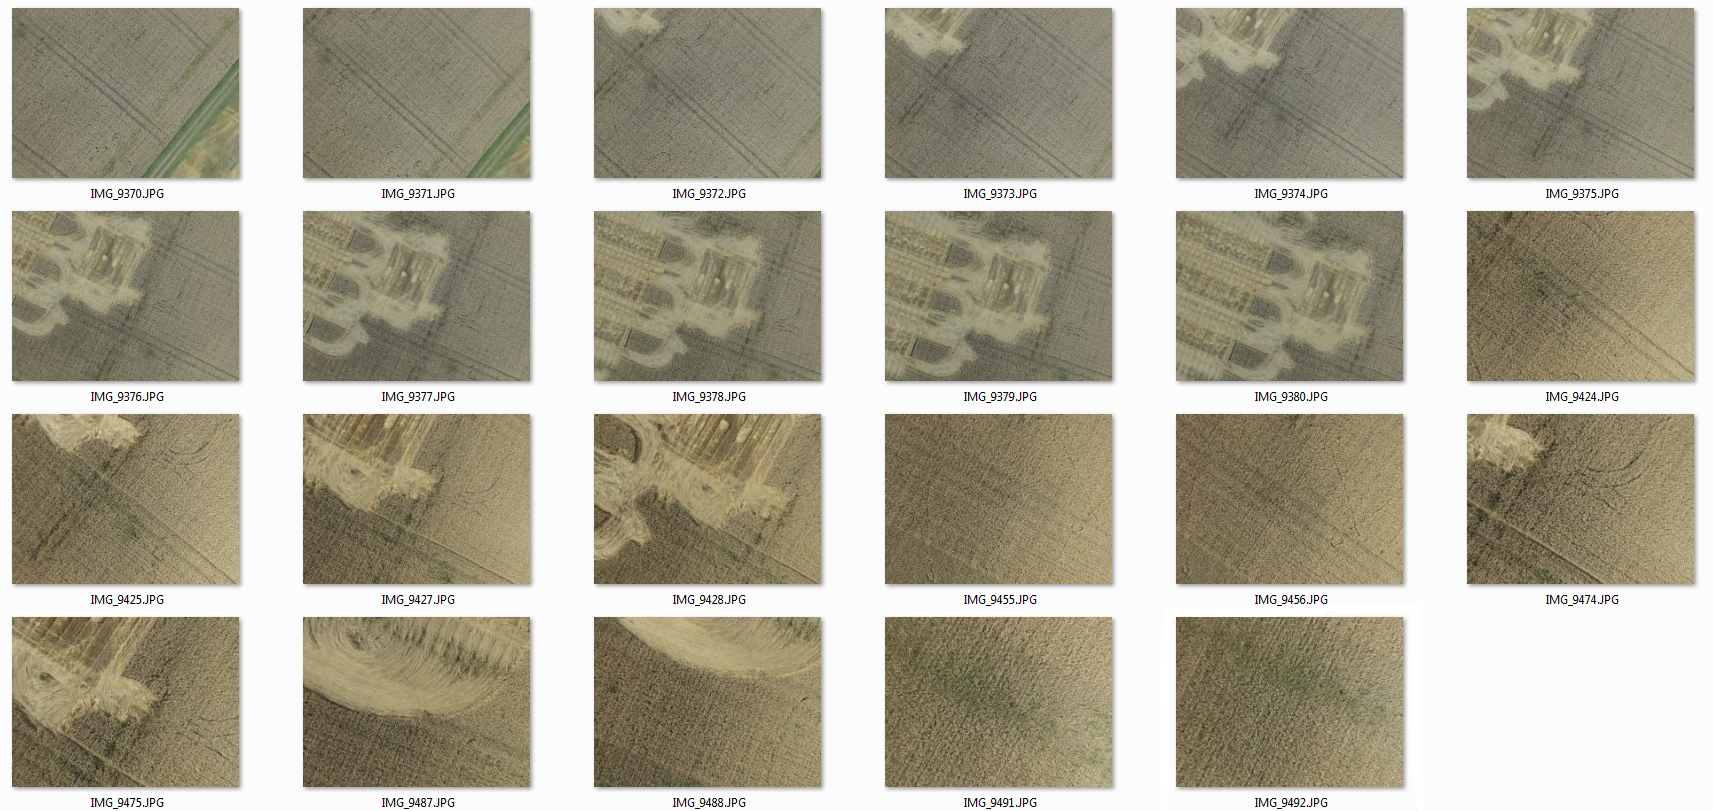
\includegraphics[width=1\textwidth]{fig/43a.png}
    \vspace{-0.5em}   
    \begin{center}
    \caption{\textcolor{gray}{\footnotesize \textit{Udvalgt billedesæt}}}
    \label{fig:lindblob}
     \end{center}
  \end{figure}
       \vspace{-2.7em}
\noindent
\section{Metode Opsætning}
Følgende er detektor/deskriptor kombinationer af beskrevne metoder, afprøvet på ovenstående billedsæt:
\begin{center}
    \begin{tabular}{ | l | l |}
    \hline
    Detektor & Deskriptor \\ \hline
    $DoG$ & SIFT <SURF?>  \\ \hline       
    Harris & SIFT \\ \hline    
    Moravec & SIFT \\ \hline    
    $DoH$ & SURF\\ \hline    
    \end{tabular}
\end{center}
Da der er blevet implementeret 4 detektorer og 2 deskriptorer, er der $4\times 2=8$ mulige metoder at afprøve. Det er her begrænset til de fire ovenstående kombinationer, <for ikke at få drukne afsnittet i tabeller>. SIFT er blevet valgt som deskriptor for metoderne, da vores undersøgelser har vist, at den giver flest matches og den højeste repeatability measure på de forskellige metoder, sammenlignet med SURF. <måske vise dette med SURF -> SIFT>
\\ \\ 
Udover de ovenstående kombinationer af metoder, er nødvendigheden for rotationsinvarians undersøgt, ved at sammenligne resultater af en rotationsinvariant deskriptor: SURF, med en ikke-rotationsinvariaant deskriptor: U-SURF. Til det er der i billedsættet udvalgt par af billeder, hvor der opstår størst rotation imellem. Disse billeder er vist i figur \ref{fig:rotation}.
\begin{center}
    \begin{tabular}{ | l | l |}
    \hline
    Detektor & Deskriptor \\ \hline
    $DoG$ & U-SURF \\ \hline       
    $DoG$ & SURF \\ \hline     
    \end{tabular}
\end{center}
Ovenstående kombination af detektor/deskriptor afprøves ikke i samme omfang som de andre kombinationer, men kun imellem to billeder, hvor der foregår stor roation imellem..
\section{Fejlkilder}
\subsection{Sortering af korrekte/ikke korrekte korrespondancer}

<FEJLKILDER>
<test kombination af billederne> \\
<hvad er testet, rotation, struktur, skala>